\documentclass[11pt]{article}
\usepackage[margin=2cm]{geometry}
\usepackage{graphicx}
\usepackage{booktabs}
\usepackage{float}
\usepackage{amsmath}
\usepackage[hidelinks]{hyperref}

\newcommand{\tab}[1]{\resizebox{\textwidth}{!}{\input{tables/#1}}}
\newcommand{\tabn}[1]{\input{tables/#1}}

\title{DMMST --- Version 2: full results\\(notebooks 01--06)}
\author{Parsa}
\date{\today}

\begin{document}
\maketitle
\tableofcontents
\newpage

%==========================================================================
\section{Summary}
We tested the components of the DMMST paper --- the numeric input embedding (\S2.2), the extra
survival losses $L_{rank}$ and $L_{mul}$ (\S2.3), and the regression (``time of event'') head with
$L_{MAE}$ and $L_{MM}$ (\S2.4) --- on five public datasets, and compared the model with eight
published survival models under one protocol.

\begin{itemize}
  \item \textbf{Accuracy.} Our model is competitive but not the best: it is in the upper half on every
        dataset and ties SurvTRACE on hsa synthetic, but wins no dataset ($C_{td}$ 0.000--0.018 behind
        the best model).
  \item \textbf{Losses.} $L_{rank}$ gives small $C_{td}$ gains on every dataset (significant only on
        hsa synthetic). The main effect of $L_{rank}$ and $L_{mul}$ is reliability: they remove failed
        splits and, on EBMT, badly calibrated ones.
  \item \textbf{Regression head.} The best-guess loss (Eq.~6) ranks predicted times better than MAE on
        observed events only, on every dataset. The head can be trained together with the survival head
        without harming it when $L_{rank}$ is used; on hsa synthetic this also improves the predicted
        times, on DeepHit synthetic it does not.
  \item \textbf{Encoding.} The paper's numeric embedding beats discretisation on METABRIC but not on
        SUPPORT. How the transformer outputs are pooled matters little, except that [CLS] is worst.
\end{itemize}

%==========================================================================
\section{Data and protocol}

\subsection{Datasets}
\begin{table}[H]
\centering
\begin{tabular}{llrll}
\toprule
Dataset & Type & Patients & Events & Source \\
\midrule
METABRIC & real & 1,904 & 1 (death) & DeepSurv release, as used by SurvTRACE \\
SUPPORT & real & 8,873 & 1 (death) & DeepSurv release, as used by SurvTRACE \\
EBMT & real & 2,279 & 4 (recovery, adverse event, relapse, death) & R package \texttt{mstate} \\
hsa synthetic & synthetic & 5,000 & 2, both can occur & Tjandra et al.\ (2021) \\
DeepHit synthetic & synthetic & 30,000 & 2, competing & Lee et al.\ (2018) \\
\bottomrule
\end{tabular}
\end{table}

\paragraph{SEER.} SEER was planned as an additional large real dataset (it is used by SurvTRACE).
Because of the updated SEER+ data-access policies we could not obtain access to it, so it is not part
of these results.

\subsection{Protocol}
The protocol follows SurvTRACE and DSM:
\begin{itemize}
  \item each dataset is split 10 times at random into 60\% train, 10\% validation and 30\% test; every
        model sees the same splits; results are mean (standard deviation) over the 10 splits;
  \item all settings are chosen on the validation split of split 0 (notebook 01); the test splits are
        used only for the final numbers;
  \item every model is scored by the same code; censoring weights and Kaplan--Meier ``best guesses'' are
        computed from the training patients of each split only.
\end{itemize}

\subsection{Metrics}
\begin{itemize}
  \item $C_{td}$: time-dependent concordance (IPCW), the mean over the 25/50/75\% quantiles of the event
        times and over events. Higher is better; 0.5 is random.
  \item Brier score at the same time points, and the integrated Brier score (IBS) and integrated
        binomial log-likelihood (IBLL) over the follow-up. Lower is better.
  \item Cumulative/dynamic AUC and Antolini's $C$ (higher is better).
  \item D-calibration $p$-value (higher means no evidence of miscalibration).
  \item For predicted times: MAE (margin and pseudo-observation versions, in the dataset's time unit) and
        Harrell's $C$ of the predicted time.
\end{itemize}

\subsection{Models}
\paragraph{Our model} is a transformer with the paper's numeric embedding and survival head
(piecewise-constant hazard). Loss recipes of the survival head:
\begin{center}
\begin{tabular}{ll}
\toprule
S1 & $L_{PCH}$ \\
S2 & $L_{PCH} + L_{rank}$ (Eq.~4) \\
S3 & $L_{PCH} + L_{mul}$ (Eq.~5) --- multi-event data only \\
S4 & $L_{PCH} + L_{rank} + L_{mul}$ --- multi-event data only \\
\bottomrule
\end{tabular}
\end{center}
Recipes of the regression head:
\begin{center}
\begin{tabular}{ll}
\toprule
R1 & $L_{MAE}$ on observed events only \\
R2 & $L_{MAE}$ with the Kaplan--Meier best guess for censored patients (Eq.~6) \\
R3 & R2 + $L_{MM}$ (Eq.~7), $t_q$ = observed time --- multi-event data only \\
R4 & R2 + $L_{MM}$, $t_q$ = best guess --- multi-event data only \\
\bottomrule
\end{tabular}
\end{center}
$L_{mul}$ and $L_{MM}$ compare different events of the same patient, so they are not defined on
single-event data (``---'' in the tables). The sign of $L_{rank}$ and $L_{mul}$ in the paper (Eqs.~4--5)
is reversed; we use the correct direction, as in DeepHit.

\paragraph{Baselines.} SurvTRACE (authors' released code), DeepHit, DSM and MENSA (on our tuned
transformer backbone), Random Survival Forest, PC-Hazard, DeepSurv and Cox. Single-event baselines are
fitted per event (cause-specific) on multi-event data.

%==========================================================================
\section{Tuning (notebook 01)}
Models were tuned on validation $C_{td}$ (24 configurations sampled from SurvTRACE's grid of 216 for
our model and SurvTRACE; full grids for Cox and RSF; 16 of 36 for DeepSurv and PC-Hazard). Loss
weights were then tuned with the chosen backbone.

\begin{table}[H]
\centering
\caption{Chosen settings of our model and of SurvTRACE (ST). lr = learning rate, wd = weight decay.}
\tab{tuned_models}
\end{table}

\begin{table}[H]
\centering
\caption{Chosen loss settings. The raw-day time unit is used only by regression-only models; models
with both heads always measure time in units of the end of follow-up (Section~\ref{sec:reg}).}
\tab{tuned_losses}
\end{table}

%==========================================================================
\section{Benchmark (notebooks 02, 03)}
Our model in this section is recipe S1 ($L_{PCH}$ only); the other recipes are compared in
Section~\ref{sec:loss}. Bold is the best per dataset.

\begin{table}[H]
\centering
\caption{$C_{td}$ (higher is better).}
\tab{bench_ctd}
\end{table}

\begin{table}[H]
\centering
\caption{Integrated Brier score (lower is better).}
\tab{bench_ibs}
\end{table}

\begin{figure}[H]
\centering
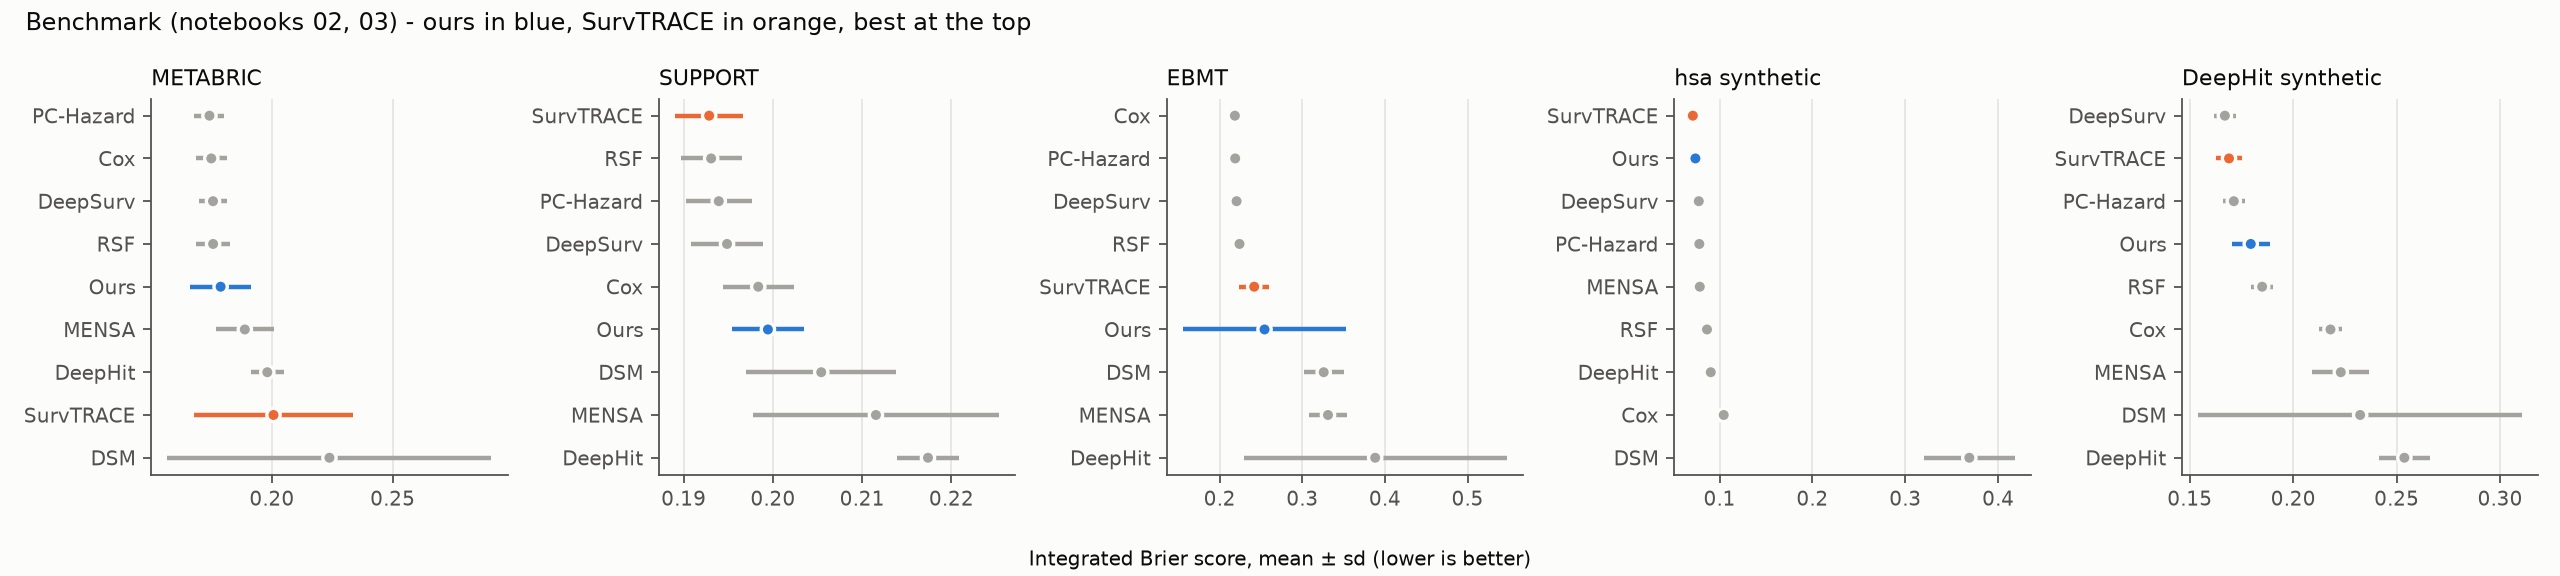
\includegraphics[width=\textwidth]{benchmark_ibs.png}
\caption{Integrated Brier score per dataset; ours in blue, SurvTRACE in orange.}
\end{figure}

\begin{table}[H]
\centering
\caption{Brier score at the 25/50/75\% time points (lower is better).}
\tab{bench_brier}
\end{table}

\begin{table}[H]
\centering
\caption{Cumulative/dynamic AUC (higher is better).}
\tab{bench_auc}
\end{table}

\begin{table}[H]
\centering
\caption{Antolini's $C$ (higher is better).}
\tab{bench_antolini}
\end{table}

\begin{table}[H]
\centering
\caption{Integrated binomial log-likelihood (lower is better).}
\tab{bench_ibll}
\end{table}

\begin{table}[H]
\centering
\caption{D-calibration $p$-value (higher = no evidence of miscalibration).}
\tab{bench_dcal}
\end{table}

\begin{table}[H]
\centering
\caption{MAE of the expected time read from the survival curve (margin MAE, linear tail; dataset time
unit; lower is better).}
\tab{bench_mae}
\end{table}

\subsection{$C_{td}$ at each time point (SurvTRACE table format)}
\begin{table}[H]
\centering
\caption{METABRIC.}
\tabn{horizons_metabric}
\end{table}
\begin{table}[H]
\centering
\caption{SUPPORT.}
\tabn{horizons_support}
\end{table}
\begin{table}[H]
\centering
\caption{EBMT, per event.}
\tab{horizons_ebmt}
\end{table}
\begin{table}[H]
\centering
\caption{hsa synthetic, per event.}
\tab{horizons_hsa_synthetic}
\end{table}
\begin{table}[H]
\centering
\caption{DeepHit synthetic, per event.}
\tab{horizons_deephit_synthetic}
\end{table}

\paragraph{Observations.}
\begin{itemize}
  \item SurvTRACE is the strongest model on METABRIC, SUPPORT and hsa synthetic; RSF and PC-Hazard on
        EBMT; DeepSurv and PC-Hazard on DeepHit synthetic. Our model (S1) is in the upper half.
  \item Our tuned SurvTRACE reproduces its published $C_{td}$ (0.678 vs 0.691 on METABRIC, 0.638 vs
        0.640 on SUPPORT), which supports the correctness of the protocol.
  \item Our calibration (IBS) is close to the best on four datasets and better than SurvTRACE's on
        METABRIC; on EBMT our IBS is high and varies between splits.
  \item DeepHit, DSM and MENSA are poorly calibrated (D-calibration $p\approx0$) and DSM and MENSA are
        unstable across splits.
  \item EBMT is hard for every model ($C_{td}$ 0.50--0.55): its four features are categorical and weak.
\end{itemize}

%==========================================================================
\section{Survival losses (notebook 05)}\label{sec:loss}

\begin{table}[H]
\centering
\caption{$C_{td}$ of each loss recipe.}
\tab{loss_ctd}
\end{table}

\begin{table}[H]
\centering
\caption{Integrated Brier score of each loss recipe.}
\tab{loss_ibs}
\end{table}

\begin{table}[H]
\centering
\caption{Brier score at the 25/50/75\% time points.}
\tab{loss_brier}
\end{table}

\begin{table}[H]
\centering
\caption{Cumulative/dynamic AUC.}
\tab{loss_auc}
\end{table}

\begin{table}[H]
\centering
\caption{Each recipe against S1 on the same 10 splits: mean difference, number of splits where the
recipe's value is higher, and paired $p$-values.}
\tab{loss_tests}
\end{table}

\begin{figure}[H]
\centering
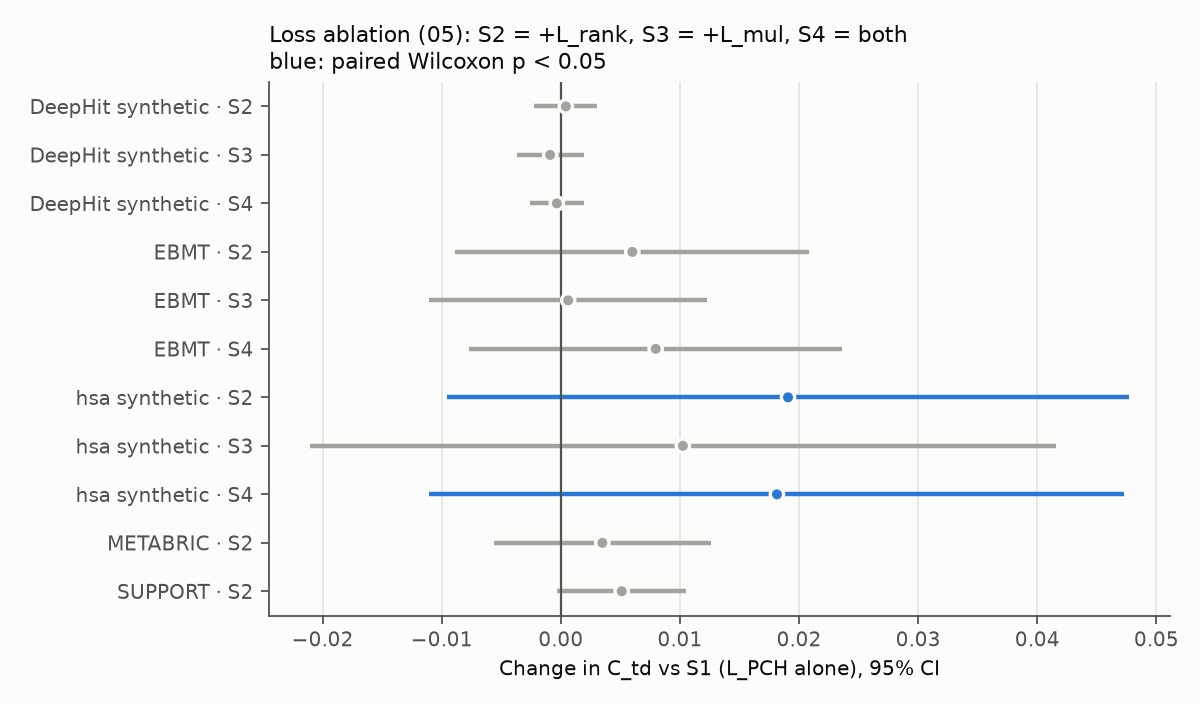
\includegraphics[width=0.75\textwidth]{losses_delta_ctd.png}
\caption{Change in $C_{td}$ against S1 with 95\% confidence intervals; blue: paired Wilcoxon $p<0.05$.}
\end{figure}

\begin{figure}[H]
\centering
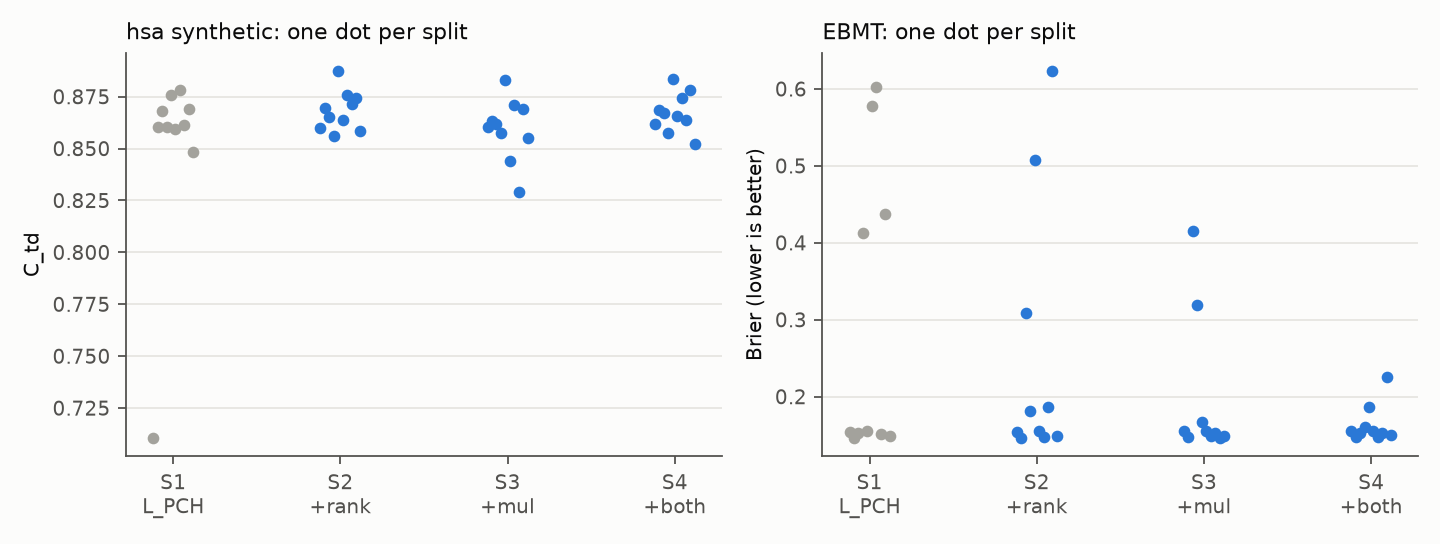
\includegraphics[width=0.85\textwidth]{losses_stability.png}
\caption{Every split of each recipe. Left: $C_{td}$ on hsa synthetic; right: Brier score on EBMT.}
\end{figure}

\paragraph{Observations.}
\begin{itemize}
  \item $L_{rank}$ (S2) is at least as good as S1 on every dataset (+0.000 to +0.019 $C_{td}$); the gain
        is significant only on hsa synthetic.
  \item $L_{mul}$ alone (S3) helps less than $L_{rank}$; S4 is about as good as S2.
  \item With $L_{PCH}$ alone, one hsa split fails ($C_{td}$ 0.71) and several EBMT splits are badly
        calibrated (Brier up to 0.6). With $L_{rank}+L_{mul}$ (S4) neither happens: the EBMT IBS drops
        from 0.338 to 0.233 and its spread from 0.165 to 0.043.
  \item On DeepHit synthetic all recipes are the same: $L_{PCH}$ alone is enough on this data.
\end{itemize}

%==========================================================================
\section{Input encoding and representation (notebook 04)}
\begin{table}[H]
\centering
\caption{Encodings of the numeric inputs and ways of pooling the transformer outputs (over layers /
over tokens / which layers).}
\tab{encoding}
\end{table}

\begin{figure}[H]
\centering
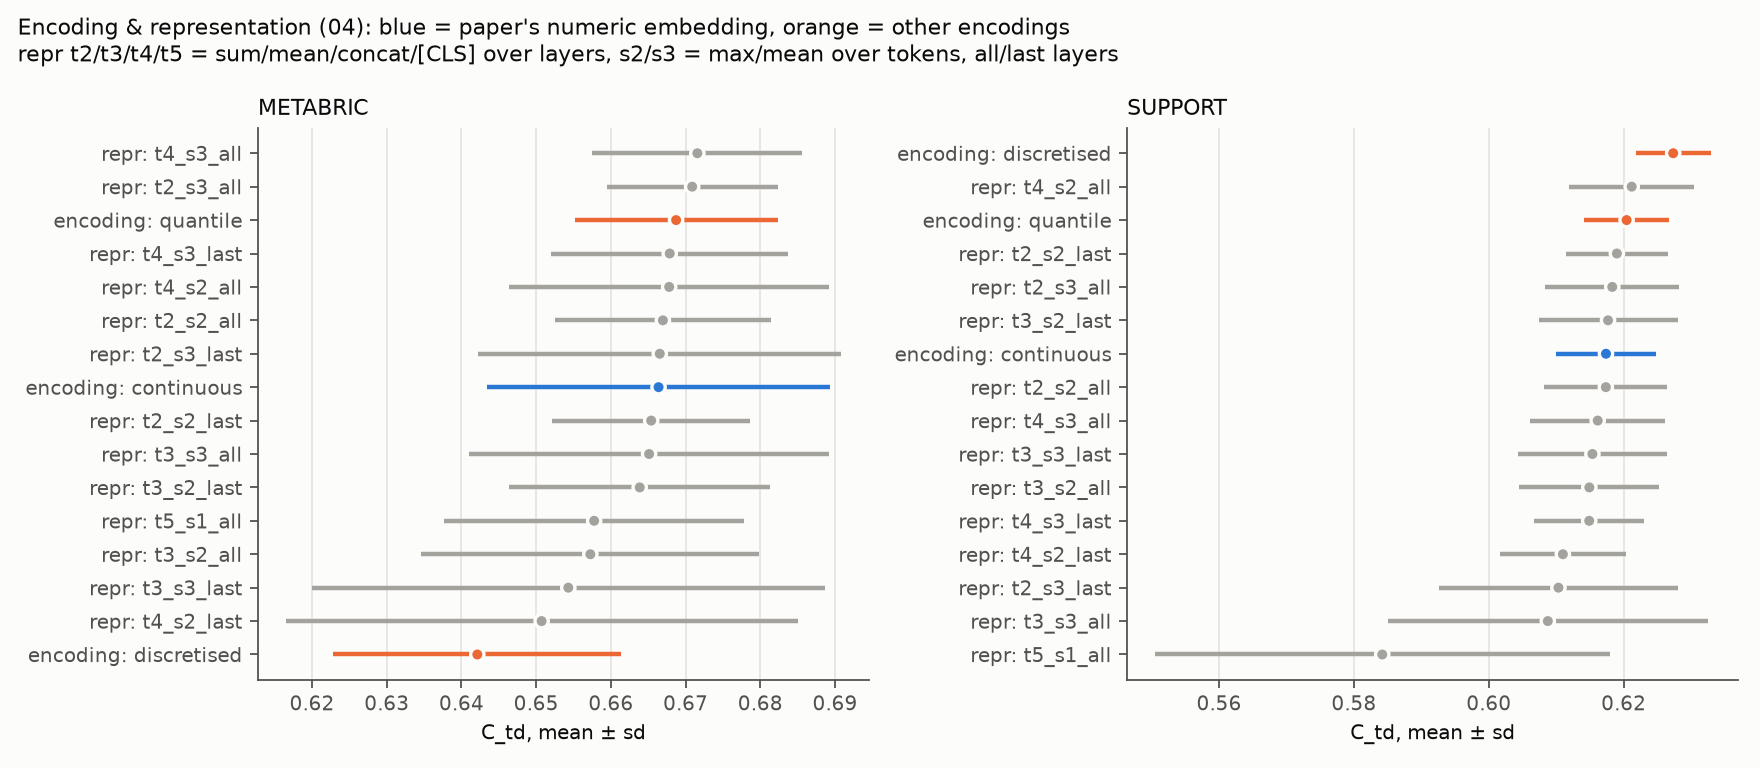
\includegraphics[width=\textwidth]{encoding_representation.png}
\caption{$C_{td}$ of every encoding and representation; blue: the paper's numeric embedding.}
\end{figure}

\paragraph{Observations.}
\begin{itemize}
  \item On METABRIC the paper's numeric embedding (0.666) is clearly better than discretisation into
        bins (0.642) and level with quantile scaling. On SUPPORT discretisation is slightly better
        (0.627 vs 0.617).
  \item Most ways of pooling the transformer outputs are within $\pm0.01$, inside the split-to-split
        spread; using the [CLS] token is clearly the worst, especially on SUPPORT.
\end{itemize}

%==========================================================================
\section{Regression head (notebook 06)}\label{sec:reg}
Two setups are trained: the regression head alone (R1--R4), and the regression head together with the
survival head (``joint'', every S $\times$ R). In joint training the time unit is the end of follow-up
and early stopping waits 30 validation rounds (Section~\ref{sec:notes}).

\begin{table}[H]
\centering
\caption{Predicted times. MAE in the dataset's time unit (lower is better); Harrell's $C$ of the predicted
time (higher is better); $C_{td}$ of the survival head for the joint models.}
\tab{regression}
\end{table}

\begin{table}[H]
\centering
\caption{Joint models on multi-event data: $C_{td}$ / Harrell's $C$ of the predicted time for every
survival recipe (rows) and regression recipe (columns).}
\tab{joint_recipes}
\end{table}

\begin{table}[H]
\centering
\caption{Joint models on single-event data: $C_{td}$ / Harrell's $C$.}
\tabn{joint_recipes_single}
\end{table}

\begin{figure}[H]
\centering
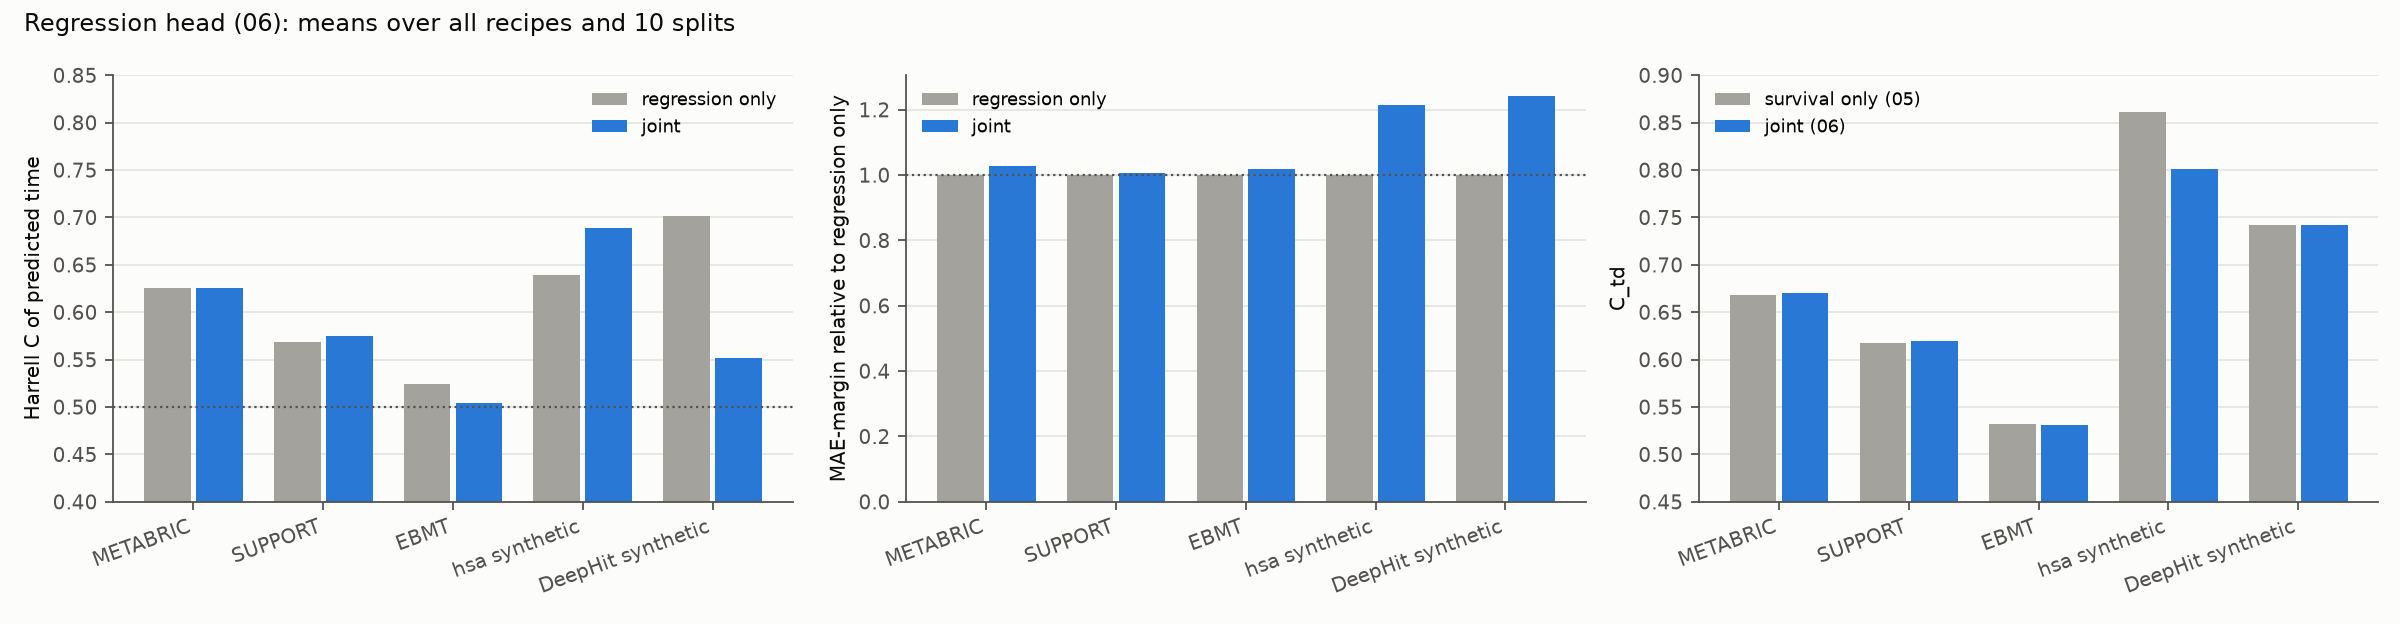
\includegraphics[width=\textwidth]{regression_head.png}
\caption{Means over all recipes and splits. Left: Harrell's $C$ of the predicted time; middle: MAE
relative to the regression-only models; right: $C_{td}$ of survival-only (notebook 05) and joint models.}
\end{figure}

\begin{figure}[H]
\centering
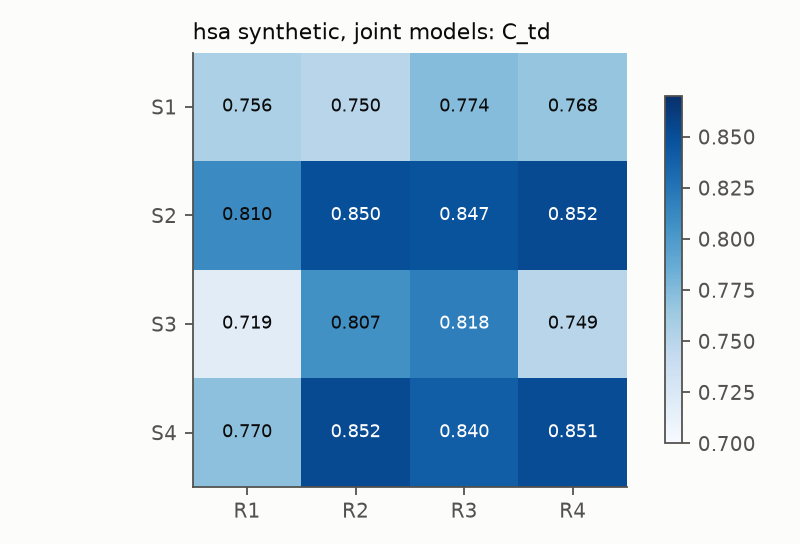
\includegraphics[width=0.45\textwidth]{joint_recipes_hsa_ctd.png}
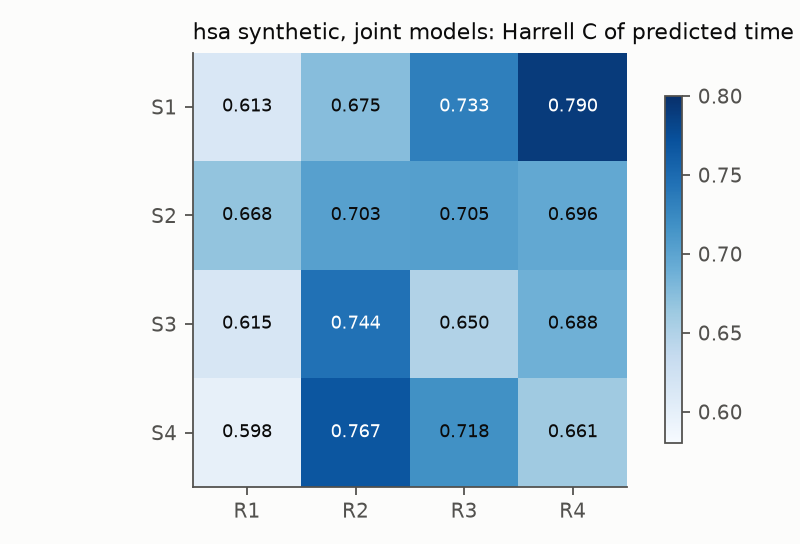
\includegraphics[width=0.45\textwidth]{joint_recipes_hsa_harrell.png}
\caption{hsa synthetic, joint models: $C_{td}$ (left) and Harrell's $C$ (right) for every recipe.}
\end{figure}

\paragraph{Observations.}
\begin{itemize}
  \item \textbf{Best guess (R2) vs observed events only (R1):} R2 ranks predicted times better on every
        dataset (Harrell's $C$, e.g.\ 0.566 $\rightarrow$ 0.663 on hsa synthetic, 0.546 $\rightarrow$
        0.592 on SUPPORT) and has a lower MAE on four of five datasets (not on hsa synthetic).
  \item \textbf{$L_{MM}$ (R3, R4)} changes little on EBMT and DeepHit synthetic; R4 is the best
        regression-only recipe on both and on hsa synthetic, by small margins.
  \item \textbf{Joint training does not harm the survival head:} $C_{td}$ equals survival-only on
        METABRIC, SUPPORT, EBMT and DeepHit synthetic. On hsa synthetic it does so only with $L_{rank}$
        (S2/S4 with R2--R4: 0.84--0.85 vs 0.86); without $L_{rank}$ (S1/S3) it is lower (0.72--0.82).
  \item \textbf{Effect on the predicted times:} on hsa synthetic the joint models rank times better than
        the regression head alone (Harrell's $C$ 0.69 on average, up to 0.79, vs 0.66). On DeepHit
        synthetic they are worse (0.55 vs 0.70): joint models choose their checkpoint by the survival
        $C_{td}$, so the regression head is not what is optimised.
  \item EBMT: predicted times carry almost no ranking information in any setup (Harrell's $C\approx0.5$).
\end{itemize}

%==========================================================================
\section{Notes on the protocol}\label{sec:notes}
\begin{itemize}
  \item \textbf{Early stopping.} Joint models can stay near $C_{td}=0.5$ for the first $\sim$30 epochs
        while the two heads settle; with a patience of 10 validation rounds some were stopped there.
        Joint models and the loss recipes of notebook 05 therefore use a patience of 30. The benchmark
        runs of notebooks 02--03 use 10; for our model (S1) the two settings agree within 0.011 $C_{td}$.
  \item \textbf{Time unit.} With raw days the regression loss (hundreds of days) dominated the survival
        loss in joint training; joint models therefore always use the end of follow-up as time unit.
  \item \textbf{Scoring fixes applied before these results:} the Brier score no longer drops patients
        censored at the last follow-up time (70\% of hsa synthetic), and IBS/IBLL/AUC are computed when a
        test patient is followed longer than every training patient.
  \item \textbf{Not included:} the language-model experiments (notebook 07, paper \S3) and sequential
        data (paper \S4.2, planned for version 3). SEER could not be used (updated SEER+ access policies).
\end{itemize}

%==========================================================================
\section{Conclusion}
Under one protocol on five public datasets, the DMMST model is competitive with strong survival models
but does not outperform SurvTRACE in $C_{td}$. The paper's additional losses are useful mainly for
reliability and calibration on multi-event data; the best-guess regression loss is better than using
observed events only; and the regression head can be trained together with the survival head without
harming it, provided $L_{rank}$ is used.

\end{document}
